\documentclass[../main.tex]{subfiles}
\begin{document}
\chapter{Integration}
\section{Basics}
We want to define $\int_{a}^{b} f(x) \d{x}$ as the signed area enclosed by $f$ between $a$ and $b$.
This is easy if the region enclosed by the graph is a nice geometric shape, if not, we can try approximating the area using rectangles.
Two ways we could do this are using the left and right Riemann sums:
\begin{center}
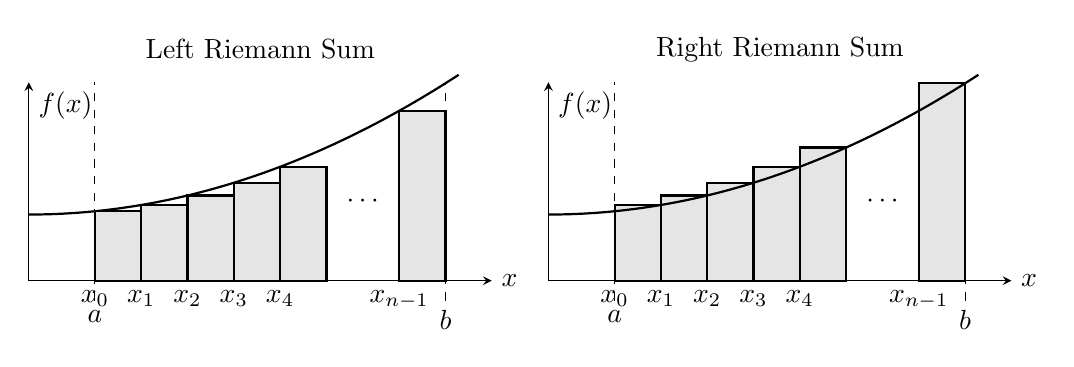
\begin{tikzpicture}[scale=1.2, >=stealth]
  \begin{scope}[scale=0.7]
    \node at (3.5, 3.5) {Left Riemann Sum};
    \draw[->] (0,0) -- (7,0) node[right] {$x$};
    \draw[->] (0,0) -- (0,3) node[below right] {$f(x)$};

    \draw[thick, domain=0:6.5, smooth, variable=\x] plot ({\x}, {0.05*\x^2 + 1});

    \node[below] at (1,-0.3) {$a$};
    \draw[dashed] (1,-0.3) -- (1,3);
    \node[below] at (6.3,-0.3) {$b$};
    \draw[dashed] (6.3,-0.3) -- (6.3,3);

    \def\dx{0.7}
    \foreach \i in {0,1,2,3,4} {
      \pgfmathsetmacro{\xleft}{1 + \i*\dx}
      \pgfmathsetmacro{\height}{0.05*\xleft^2 + 1}
      \fill[gray!20] (\xleft,0) rectangle ({\xleft+\dx}, {\height});
      \draw[thick] (\xleft,0) rectangle ({\xleft+\dx}, {\height});
      \node[below] at (\xleft,0) {$x_\i$};
    }

    \node at (5.05,1.2) {$\cdots$};

    \pgfmathsetmacro{\xfinal}{5.6}
    \pgfmathsetmacro{\hfinal}{0.05*\xfinal^2 + 1}
    \node[below] at (\xfinal,0) {$x_{n-1}$};
    \fill[gray!20] (\xfinal,0) rectangle ({\xfinal+\dx}, {\hfinal});
    \draw[thick] (\xfinal,0) rectangle ({\xfinal+\dx}, {\hfinal});
  \end{scope}

  \begin{scope}[xshift=5.5cm, scale=0.7]
    \node at (3.5, 3.5) {Right Riemann Sum};
    \draw[->] (0,0) -- (7,0) node[right] {$x$};
    \draw[->] (0,0) -- (0,3) node[below right] {$f(x)$};


    \node[below] at (1,-0.3) {$a$};
    \draw[dashed] (1,-0.3) -- (1,3);
    \node[below] at (6.3,-0.3) {$b$};
    \draw[dashed] (6.3,-0.3) -- (6.3,3);

    \def\dx{0.7}
    \foreach \i in {0,1,2,3,4} {
      \pgfmathsetmacro{\xleft}{1 + \i*\dx}
      \pgfmathsetmacro{\height}{0.05*(\xleft + \dx)^2 + 1}
      \fill[gray!20] (\xleft,0) rectangle ({\xleft+\dx}, {\height});
      \draw[thick] (\xleft,0) rectangle ({\xleft+\dx}, {\height});
      \node[below] at (\xleft,0) {$x_\i$};
    }

    \node at (5.05,1.2) {$\cdots$};

    \pgfmathsetmacro{\xfinal}{5.6}
    \pgfmathsetmacro{\hfinal}{0.05*(\xfinal + \dx)^2 + 1}
    \node[below] at (\xfinal,0) {$x_{n-1}$};
    \fill[gray!20] (\xfinal,0) rectangle ({\xfinal+\dx}, {\hfinal});
    \draw[thick] (\xfinal,0) rectangle ({\xfinal+\dx}, {\hfinal});

    \draw[thick, domain=0:6.5, smooth, variable=\x] plot ({\x}, {0.05*\x^2 + 1});
  \end{scope}
\end{tikzpicture}
\end{center}
We first need to define how we can split up the real line between the \textit{integration bounds $a$ and $b$}:
\begin{definition}[Partition/Dissection]
  A \textit{partition} $\mathcal{P}$ or \textit{dissection} of an interval $[a, b]$ is a \textbf{finite subset} of $[a, b]$ with the requirement that $a, b \in \mathcal{P}$.

  We often write $\mathcal{P} = \{x_0, \ldots, x_n\}$ where $a = x_0 < x_1 < \cdots < x_n = b$ and $x_i \in [a, b]\ \forall i$.
\end{definition}
Instead of the left and right Riemann sums, we will instead use the \textit{upper and lower} Riemann sums.
These use the supremum/infimum respectively of $f$ over each interval between the points of a partition.
\begin{definition}[Upper/Lower Riemman Sums]
  For a bounded $f: [a, b] \to \R$ and partition $\mathcal{P}$ of $[a, b]$, we define the \textit{Lower Riemann sum} as:
  \[
    L(f, \mathcal{P}) = \sum_{j = 1}^{n} (x_j - x_{j - 1}) \inf_{x \in I_j} f(x)
  \]
  and the \textit{Upper Riemann sum} as:
  \[
    U(f, \mathcal{P}) = \sum_{j = 1}^{\infty} (x_j - x_{j - 1}) \sup_{x \in I_j} f(x)
  \]
  where $I_j = [x_{j - 1}, x_{j}]$.
\end{definition}
\begin{example}
  Consider again the \textit{Dirichlet function} from \cref{dirichletFunction}:
  \label{dirichletUpperLower}
  \[
    f(x) = 1_\Q(x) = \begin{cases}
    1 & \text{ if } x \in \Q \\
    0 & \text{ if } x \notin \Q
    \end{cases}
  \]
  No matter what $\mathcal{P}$ is, since $\Q$ is dense in $\R$, $I_j = [x_{j - 1}, x_j]$ will always contain a rational and an irrational number, hence:
  \[
    \sup_{x \in I_j} f(x) = 1 \text{ and } \inf_{x \in I_j} f(x) = 1
  \]
  and so:
  \begin{align*}
    U(f, \mathcal{P}) &= 1 \cdot \sum_{j = 1}^{n} (x_j - x_{j - 1}) \\
                       &= x_1 - x_0 + x_2 - x_1 + \cdots + x_n - x_{n - 1} \\
                       &= x_n - x_0 = b - a = 1 - 0 = 1 \\
    L(f, \mathcal{P}) &= 0 \cdot \sum_{j = 1}^{n} (x_j - x_{j - 1}) = 0 \\
  \end{align*}
\end{example}
For bounded $f$, $\exists k \text{ s.t. } \sup_{x \in [a, b]} |f(x)| = k$.
Since $\sup_{x \in I_j} f(x) \leq \sup_{x \in [a, b]} f(x)$, we can bound $U(f, \mathcal{P})$ as:
\begin{align*}
  U(f, \mathcal{P}) &\leq \sum_{j = 1}^{n} (x_{j} - x_{j - 1}) \sup_{x \in [a, b]} |f(x)|  \\
                     &\leq K \sum_{j = 1}^{n} (x_j - x_{j - 1}) = k(b - a)
\end{align*}
and since $\inf_{x \in I_j} f(x) \geq \inf_{x \in [a, b]} f(x) \geq -\sup_{x \in [a, b]} |f(x)| = -k$
\begin{align*}
  L(f, \mathcal{P}) &\geq \sum_{j = 1}^{n} (x_{j} - x_{j -1}) \left[- \sup_{x \in [a, b]} |f(x)|\right] \\
                     &= -k(b - a)
\end{align*}
From the definition, we clearly have that $U(f, \mathcal{P}) \geq L(f, \mathcal{P})$ and so:
\[
  -k(b - a) \leq L(f, \mathcal{P}) \leq U(f, \mathcal{P}) \leq k(b - a)
\]
Geometrically, this is saying that $L$ and $U$ are bounded below by a rectangle from $a$ to $b$ of height $-k$ and above by a rectangle from $a$ to $b$ of height $k$ where $k = \sup_{x \in [a, b]} f(x)$.

Therefore, the sets:
\[
  \{L(f, \mathcal{P}): \mathcal{P} \text{ is a partition of $[a, b]$}\} \text{ and } \{U(f, \mathcal{P}): \mathcal{P} \text{ is a partition of $[a, b]$}\}
\]
are both bounded.
They are also non empty since as $\{a,b\}$ is always a partition of $[a, b]$.
This means that they both have supremum and infimum.
\begin{definition}[Upper/Lower Integral]
  Let $f: [a, b] \to \R$ be a bounded function.
  We define the \textit{lower Riemann integral} of $f$ in $[a, b]$ as:
  \[
    I_{*}(f) = \sup_{\mathcal{P}} L(f, \mathcal{P})
  \]
  and the \textit{upper Riemann integral} of $f$ in $[a, b]$ as:
  \[
    I^{*}(f) = \inf_{\mathcal{P}} U(f, \mathcal{P})
  \]
\end{definition}
\begin{definition}[Riemman Integrable]
  We say that bounded function $f: [a, b] \to \R$ is \textit{Riemann integrable} if $I_{*}(f) = I^{*}(f)$ and then define:
  \[
    I(f) = \int_{a}^{b} f(x) \d{x} = I_{*}(f) = I^{*}(f)
  \]
  to be the \textit{Riemann integral of $f$ from $a$ to $b$}.
\end{definition}
\begin{remark}
  If we change the order of the bounds, then the sign of the integral flips, that is:
  \[
    \int_{a}^{b} f(x) \d{x} = - \int_{b}^{a} f(x) \d{x}
  \]
\end{remark}
\begin{example}
  Consider the dirichlet indicator function from \cref{dirichletUpperLower} again.
  Its upper and lower integrals are $I^{*}(f) = 1$ and $I_{*}(f) = 0$, so $f$ is not integrable.
\end{example}
\end{document}
